\documentclass[12 pt]{amsart}
\usepackage{amsmath, amssymb, amsthm,amscd}
\usepackage{float}
\usepackage{tkz-graph}
\usepackage{tikz}
\usepackage{tikz,fullpage}
\usetikzlibrary{positioning, quotes}
\usetikzlibrary{calc,arrows,petri,topaths}
\usetikzlibrary{graphs,quotes}
\usepackage[latin1]{inputenc}
\usepackage{tkz-berge}
\usepackage[position=top]{subfig}

\allowdisplaybreaks

\newcommand{\mathsym}[1]{{}}
\newcommand{\unicode}{{}}

\newtheorem{theorem}{Theorem}[section]
\newtheorem{lemma}[theorem]{Lemma}
\newtheorem{proposition}[theorem]{Proposition}
\newtheorem{corollary}[theorem]{Corollary}
\newtheorem{definition}[theorem]{Definition}
\newtheorem{construction}[theorem]{Construction}

\newcommand\T{\rule{0pt}{-1.0ex}}       % Top strut
\newcommand\B{\rule[0.5ex]{0pt}{0pt}} % Bottom strut

\newcommand{\smat}[4] {(\begin{smallmatrix} #1 & #2 \\ #3 & #4 \end{smallmatrix} )}
\newcommand{\mat}[4]  { \left(\begin{array}{cc} #1 & #2 \\ #3 & #4 \end{array} \right)}
\newcommand{\schar}[2] {( \begin{smallmatrix} #1 \\ #2 \end{smallmatrix})}

\newcommand{\op}[1]  { \operatorname{ #1 }}
\newcommand{\olbbH}[0]  { \overline{\mathbb{H}}}
\newcommand{\olbbQ}[0]  { \overline{\mathbb{Q}}}
\newcommand{\olG}[0]  { \overline{\Gamma}}
\newcommand{\bbH}[0]  { \mathbb{H}}
\newcommand{\bbC}[0]  { \mathbb{C}}
\newcommand{\bbZ}[0]  { \mathbb{Z}}
\newcommand{\bbF}[0]  { \mathbb{F}}
\newcommand{\bbQ}[0]  { \mathbb{Q}}
\newcommand{\bbR}[0]  { \mathbb{R}}
\newcommand{\gok}[0]  { \mathfrak{k}}
\newcommand{\goe}[0]  { \mathfrak{e}}
\newcommand{\goR}[0]  { \mathfrak{R}}

\newcommand{\om}[2] {\omega_{#1}^{#2}}

\usepackage{bbm}
\newcommand{\ee}[0] {\mathbbm{e}}
\newcommand{\ii}[0] {\mathbbm{i}}

%\newcommand{\ee}[0] {e}
%\newcommand{\ii}[0] {i}

\addtolength{\textwidth}{1.0in}
\addtolength{\hoffset}{-0.6in}
\addtolength{\textheight}{0.6in}
\addtolength{\voffset}{-0.3in}

\begin{document}
\title{fft}
\maketitle

\begin{abstract}
beefy floating point units
\end{abstract}

\section{notation}

\begin{tabular}{l|l}
$\ii$ & $\sqrt{-1}$ \\
$\ee$ & $2.71\dots$ \\
$\pi$ & $3.14\dots$ \\
$\operatorname{EvalPoly}(a, \vec{x})$ & $\sum_{0 \le i < n} x_i a^i$, $\vec{x} = (x_0, \dots, x_{n-1})$\\
$\om{b}{a}$ & $\ee^{2 a \pi \ii / b}$ when the base ring is $\mathbb{C}$, 
Otherwise some compatible $b^{\text{th}}$ root of unity.\\
$\overline{i}^k$ & length $k$ bit-reversal of $i$. Only defined for $0 \le i < 2^k$\\
\end{tabular} 

\section{fft/ifft}

\subsection{Bit Reversal}

Unless the output of the fft is specifically needed to be in the usual order
\begin{equation*}
\left\{\operatorname{EvalPoly}(\om{2^k}{i}, \vec{x})\right\}_{0 \le i < 2^k}
\end{equation*}
there is no reason not to give the output in bit-reversed order
\begin{equation*}
\left\{\operatorname{EvalPoly}(\om{2^k}{\overline{i}^k}, \vec{x})\right\}_{0 \le i < 2^k}\text{.}
\end{equation*}
The reason is that the bit-reversed output is much simpler and faster because it
groups similar outputs close together. For example, $\operatorname{EvalPoly}(1, \vec{x})$ and
$\operatorname{EvalPoly}(-1, \vec{x})$ are very similar computationally and are right next to
each other in the bit-reversed output, but are very far apart in the usual order. Therefore,
we will restrict exclusively to bit-reversed outputs.


The usual sequence for calculating a length $16$ fft follows the columns below and ends with
the fft in the last column.
\begin{equation}
\label{ifft_fma}
\begin{tabular}{c|c|c|c|c}
$x_i$ & $y_i$ & $z_i$ & $w_i$ & $\operatorname{fft}(\vec{x})$\\
\hline
 $x_{0}$ &  $x_{0}+x_{8}$              & $y_{0}+y_{4}$              & $z_{0}+z_{2}$              & $w_{0} + w_{1}$\T\B\\
 $x_{1}$ &  $x_{1}+x_{9}$              & $y_{1}+y_{5}$              & $z_{1}+z_{3}$              & $(w_{0} - w_{1})$\T\B\\
 $x_{2}$ &  $x_{2}+x_{10}$             & $y_{2}+y_{6}$              & $(z_{0}-z_{2})\om{4}{0}$   & $w_{2} + w_{3}$\T\B\\
 $x_{3}$ &  $x_{3}+x_{11}$             & $y_{3}+y_{7}$              & $(z_{2}-z_{3})\om{4}{1}$   & $(w_{2} - w_{3})$\T\B\\
 $x_{4}$ &  $x_{4}+x_{12}$             & $(y_{0}-y_{4})\om{8}{0}$   & $z_{4}+z_{6}$              & $w_{4} + w_{5}$\T\B\\
 $x_{5}$ &  $x_{5}+x_{13}$             & $(y_{1}-y_{5})\om{8}{1}$   & $z_{5}+z_{7}$              & $(w_{4} - w_{5})$\T\B\\
 $x_{6}$ &  $x_{6}+x_{14}$             & $(y_{2}-y_{6})\om{8}{2}$   & $(z_{4}-z_{6})\om{4}{0}$   & $w_{6} + w_{7}$\T\B\\
 $x_{7}$ &  $x_{7}+x_{15}$             & $(y_{3}-y_{7})\om{8}{3}$   & $(z_{5}-z_{7})\om{4}{1}$   & $(w_{6} - w_{7})$\T\B\\
 $x_{8}$ &  $(x_{0}-x_{8})\om{16}{0}$  & $y_{8}+y_{12}$             & $z_{8}+z_{10}$             & $w_{8} + w_{9}$\T\B\\
 $x_{9}$ &  $(x_{1}-x_{9})\om{16}{1}$  & $y_{9}+y_{13}$             & $z_{9}+z_{11}$             & $(w_{8} - w_{9})$\T\B\\
$x_{10}$ &  $(x_{2}-x_{10})\om{16}{2}$ & $y_{10}+y_{14}$            & $(z_{8}-z_{10})\om{4}{0}$  & $w_{10} + w_{11}$\T\B\\
$x_{11}$ &  $(x_{3}-x_{11})\om{16}{3}$ & $y_{11}+y_{15}$            & $(z_{9}-z_{11})\om{4}{1}$  & $(w_{10} - w_{11})$\T\B\\
$x_{12}$ &  $(x_{4}-x_{12})\om{16}{4}$ & $(y_{8}-y_{12})\om{8}{0}$  & $z_{12}+z_{14}$            & $w_{12} + w_{13}$\T\B\\
$x_{13}$ &  $(x_{5}-x_{13})\om{16}{5}$ & $(y_{9}-y_{13})\om{8}{1}$  & $z_{13}+z_{15}$            & $(w_{12} - w_{13})$\T\B\\
$x_{14}$ &  $(x_{6}-x_{14})\om{16}{6}$ & $(y_{10}-y_{14})\om{8}{2}$ & $(z_{12}-z_{14})\om{4}{0}$ & $w_{14} + w_{15}$\T\B\\
$x_{15}$ &  $(x_{7}-x_{15})\om{16}{7}$ & $(y_{11}-y_{15})\om{8}{3}$ & $(z_{13}-z_{15})\om{4}{1}$ & $(w_{14} - w_{15})$\T\B\\
\end{tabular} 
\end{equation}
One problem with this approach is that each column accesses many different
\emph{twiddle factors} $\omega_b^a$. In the case of a Sch\"onhage--Strassen fft where the base
ring is $\mathbb{Z}/(2^{m}+1)\mathbb{Z}$, this doesn't matter because each twiddle factor is a
power of two and implemented via bit shifts. In other cases, these twiddle factors have to be
either computed on the fly or precomputed and then retrieved from storage. In the case of precomputation,
we have to have in memory the table
\begin{equation}
\label{ifft_fma_tab}
1,\om{2}{1}, 1,\om{4}{1}, 1, \om{8}{1}, \om{8}{2}, \om{8}{3}, 1, \om{16}{1}, \om{16}{2}, \om{16}{3}, \om{16}{4}, \om{16}{5}, \om{16}{6}, \om{16}{7}, 1, \dots
\end{equation}
so that the columns can access this table sequentially. However, such a table is nice because
once it is extended to accommodate an fft of a certain length, it can be reused 
for all ffts of
smaller length.

By rearranging the twiddle factors as ($\omega = \omega_{16}$)

\begin{equation}
\label{fft_fma}
\begin{tabular}{c|c|c|c|c}
$x_i$ & $y_i$ & $z_i$ & $w_i$ & $\operatorname{fft}(\vec{x})$\\
\hline
 $x_{0}$ &  $x_{0}+\om{}{0}x_{8}$  & $y_{0}+\om{}{0}y_{4}$    & $z_{0}+\om{}{0}z_{2}$    & $w_{0}+\om{}{0}w_{1}$\T\B\\
 $x_{1}$ &  $x_{1}+\om{}{0}x_{9}$  & $y_{1}+\om{}{0}y_{5}$    & $z_{1}+\om{}{0}z_{3}$    & $w_{0}+\om{}{8}w_{1}$\T\B\\
 $x_{2}$ &  $x_{2}+\om{}{0}x_{10}$ & $y_{2}+\om{}{0}y_{6}$    & $z_{0}+\om{}{8}z_{2}$    & $w_{2}+\om{}{4}w_{3}$\T\B\\
 $x_{3}$ &  $x_{3}+\om{}{0}x_{11}$ & $y_{3}+\om{}{0}y_{7}$    & $z_{1}+\om{}{8}z_{3}$    & $w_{2}+\om{}{12}w_{3}$\T\B\\
 $x_{4}$ &  $x_{4}+\om{}{0}x_{12}$ & $y_{0}+\om{}{8}y_{4}$    & $z_{4}+\om{}{4}z_{6}$    & $w_{4}+\om{}{2}w_{5}$\T\B\\
 $x_{5}$ &  $x_{5}+\om{}{0}x_{13}$ & $y_{1}+\om{}{8}y_{5}$    & $z_{5}+\om{}{4}z_{7}$    & $w_{4}+\om{}{10}w_{5}$\T\B\\
 $x_{6}$ &  $x_{6}+\om{}{0}x_{14}$ & $y_{2}+\om{}{8}y_{6}$    & $z_{4}+\om{}{12}z_{6}$   & $w_{6}+\om{}{6}w_{7}$\T\B\\
 $x_{7}$ &  $x_{7}+\om{}{0}x_{15}$ & $y_{3}+\om{}{8}y_{7}$    & $z_{5}+\om{}{12}z_{7}$   & $w_{6}+\om{}{14}w_{7}$\T\B\\
 $x_{8}$ &  $x_{0}+\om{}{8}x_{8}$  & $y_{8}+\om{}{4}y_{12}$   & $z_{8}+\om{}{2}z_{10}$   & $w_{8}+\om{}{1}w_{9}$\T\B\\
 $x_{9}$ &  $x_{1}+\om{}{8}x_{9}$  & $y_{9}+\om{}{4}y_{13}$   & $z_{9}+\om{}{2}z_{11}$   & $w_{8}+\om{}{9}w_{9}$\T\B\\
$x_{10}$ &  $x_{2}+\om{}{8}x_{10}$ & $y_{10}+\om{}{4}y_{14}$  & $z_{8}+\om{}{10}z_{10}$  & $w_{10}+\om{}{5}w_{11}$\T\B\\
$x_{11}$ &  $x_{3}+\om{}{8}x_{11}$ & $y_{11}+\om{}{4}y_{15}$  & $z_{9}+\om{}{10}z_{11}$  & $w_{10}+\om{}{13}w_{11}$\T\B\\
$x_{12}$ &  $x_{4}+\om{}{8}x_{12}$ & $y_{8}+\om{}{12}y_{12}$  & $z_{12}+\om{}{6}z_{14}$  & $w_{12}+\om{}{3}w_{13}$\T\B\\
$x_{13}$ &  $x_{5}+\om{}{8}x_{13}$ & $y_{9}+\om{}{12}y_{13}$  & $z_{13}+\om{}{6}z_{15}$  & $w_{12}+\om{}{11}w_{13}$\T\B\\
$x_{14}$ &  $x_{6}+\om{}{8}x_{14}$ & $y_{10}+\om{}{12}y_{14}$ & $z_{12}+\om{}{14}z_{14}$ & $w_{14}+\om{}{7}w_{15}$\T\B\\
$x_{15}$ &  $x_{7}+\om{}{8}x_{15}$ & $y_{11}+\om{}{12}y_{15}$ & $z_{13}+\om{}{14}z_{15}$ & $w_{14}+\om{}{15}w_{15}$\T\B\\
\end{tabular} 
\end{equation}
there are still the same number of twiddle factor multiplications, but each twiddle factor
itself can be reused in each column. Also, as with the previous method, there is a
universal (bit-reversed) table
\begin{equation}
\label{fft_fma_tab}
1,
\quad \om{2}{1},
\quad \om{4}{1}, \om{4}{3},
\quad \om{8}{1},\om{8}{5},\om{8}{3},\om{8}{7},
\quad \om{16}{1},\om{16}{9},\om{16}{5},\om{16}{13},\om{16}{3},\om{16}{11},\om{16}{7},\om{16}{15},
\quad \dots
\end{equation}
that can be reused. The difference here is that the portion that is used for a
specific fft is now half the size (making note of $\om{4}{3} = -\om{4}{1}$,
$\om{8}{5} = -\om{8}{1}$, $\om{8}{7} = -\om{8}{3}$, etc.).

Since the output of the fft is given in bit-reversed order, the inverse
operation cannot simply replace $\omega$ by $\omega^{-1}$ and use the same
calculation sequence. Thus the ifft has to invert the left-to-right operation
by working from the right to the left and inverting each basic operation. This
gives slightly different data access patterns but involves essentially the same
calculations. For example, the operation $w_8 = z_8 + \omega^2 z_{10}\text{,}
\, w_{10} = z_8 - \omega^2 z_{10}$ is inverted by $2 z_8 = w_8 + w_{10}\text{,}
\, 2 z_{10} = \omega^{-2}(w_8 - w_{10})$ and the negative power
$\omega^{-\overline{i}^k}$ can be looked up in the table by flipping all bits
of $i$ except the highest.

\subsection{fft on sizes other than powers of two}
\label{section_odd}

Suppose the vector to transform has length thrice a power of two: 
$x_0,x_1,\dots,x_{3\cdot2^k-1}$. If, for each $0 \le i < 2^k$, we first perform
\begin{align*}
y_{i}^{(0)} &= x_{i+0\cdot 2^k} + x_{i+1\cdot 2^k} + x_{i+2\cdot 2^k}\\
y_{i}^{(1)} &= \om{3\cdot 2^k}{i}(x_{i+0\cdot 2^k} + \om{3}{1}x_{i+1\cdot 
2^k} + \om{3}{-1}x_{i+2\cdot 2^k})\\
y_{i}^{(2)} &= \om{3\cdot 2^k}{-i}(x_{i+0\cdot 2^k} + 
\om{3}{-1}x_{i+1\cdot 
2^k} + \om{3}{1}x_{i+2\cdot 2^k})\text{,}
\end{align*}
then the three ffts of the length $2^k$ sequences $y^{(0)}, y^{(1)}, y^{(2)}$ 
will give the fft of the original sequence. However, while the transforms
of $y^{(0)}$ and $y^{(1)}$ will have the same ordering, the sequence $y^{(2)}$
will transform to a different ordering due to the negative power.
More precisely,
\begin{align*}
\operatorname{EvalPoly}(\om{3\cdot2^k}{3i}, x) &= 
\operatorname{EvalPoly}(\om{2^k}{i}, y^{(0)})\\
\operatorname{EvalPoly}(\om{3\cdot2^k}{3i+1}, x) &= 
\operatorname{EvalPoly}(\om{2^k}{i}, y^{(1)})\\
\operatorname{EvalPoly}(\om{3\cdot2^k}{3i-1}, x) &= 
\operatorname{EvalPoly}(\om{2^k}{i}, y^{(2)})\text{.}
\end{align*}


\subsection{Considerations for the base ring $\mathbb{C}$}
\label{section_CC}
When arithmetic in the base ring necessarily includes roundoff error, it is
important for the fft to be implemented as accurately as possible. Since both
\eqref{ifft_fma} and \eqref{fft_fma} compute the bit-reversed fft, we are free
to use either. Using \eqref{fft_fma} for the forward transform and inverting
\eqref{ifft_fma} for the inverse transform gives calculation sequences for both
that consist \emph{entirely of fused-multiply-add operations}. The ifft will
read often from the table \eqref{ifft_fma_tab}, but this is of little
consequence since large convolution lengths are not feasible for this base ring
(see Table \ref{doubles_suck}).
\begin{table}
\caption{Integer multiplication with complex $53$ bit ffts: The two input
numbers are viewed as polynomials evaluated at $2^m$ so that the fft has inputs
in the range $[0,2^m)$. The output coefficients from the ifft are eventually
unreliable due to rounding errors: let $f(m)$ denote the maximum
bit size of an answer which can be guaranteed correct by this algorithm.}
\label{doubles_suck}
\begin{tabular}{r|l}
$m$ & upper bound on $f(m)$\\
\hline
$22$ & $3008$\T\B\\
$21$ & $11968$\T\B\\
$20$ & $30464$\T\B\\
$19$ & $117632$\T\B\\
$18$ & $417280$\T\B\\
$17$ & $1246592$\T\B\\
$16$ & $1984000$\T\B
\end{tabular} 
\end{table}
One further issue that arises in some possible implementations is a $n$-fold
increase in the size of the twiddle tables when processing with $n$-wide
vectors. Since the tables \eqref{fft_fma_tab} or \eqref{ifft_fma_tab} are used
only for the calculations in lane number $0$, there must be $n-1$ ``twists'' of
this data available for the other vector lanes.

The case of real input and output data is important and can be
optimized. Feeding in purely real data to the fft and getting back real data
from the ifft represents only a 50\% utilization of the circuits 
\eqref{ifft_fma} or \eqref{fft_fma}, since the data possesses certain 
symmetries under complex conjugation in each column of the calculation.
First, and most elementary, two real data sets $\vec{a}$ and $\vec{b}$ of the
same length can be transformed with one complex transformation of the same
length, and this is nothing but the linearity of the fft operation:
\begin{align*}
\operatorname{EvalPoly}(\omega, \vec{a} + \ii \vec{b}) = 
\operatorname{EvalPoly}(\omega,\vec{a}) + \ii 
\operatorname{EvalPoly}(\omega,\vec{b})\\
\overline{\operatorname{EvalPoly}(\omega^{-1}, \vec{a} + \ii \vec{b})} = 
\operatorname{EvalPoly}(\omega,\vec{a}) - \ii 
\operatorname{EvalPoly}(\omega,\vec{b})
\end{align*}
This is fine for doubling the processing speed of an even number of data sets 
of the same length, but if we would like to process one data set twice as fast,
the following identity can be used.
\begin{equation*}
\operatorname{EvalPoly}(\omega, (x_0,\dots,x_{2n-1})) = \operatorname{EvalPoly}(\omega^2, (x_0, x_2,\dots,x_{2n-2})) + \omega \operatorname{EvalPoly}(\omega^2, (x_1, x_3,\dots,x_{2n-1}))\text{.}
\end{equation*}
Multiplication of real coefficients $\{a_i\}$ and $\{b_i\}$ to
form product coefficients $\{c_i\}$ can then take the form
\begin{equation*}
\begin{array}{c}
a_0 + \ii b_0\\
a_1 + \ii b_1\\
\dots\\
a_{15} + \ii b_{15}\\
\end{array}
\underset{\operatorname{fft}_{16}}{\Longrightarrow}
\begin{array}{l}
{f}_{0}\\
{f}_{8}\\
{f}_{4}\\
{f}_{12}\\
\dots\\
{f}_{14}\\
{f}_{1}\\
\dots\\
{f}_{7}\\
{f}_{15}\end{array}
\Longrightarrow
\begin{array}{r}
\hat{a}_{0} \cdot \hat{b}_{0} = \hat{c}_{0}\\
\hat{a}_{8} \cdot \hat{b}_{8} = \hat{c}_{8}\\
\hat{a}_{4} \cdot \hat{b}_{4} = \hat{c}_{4}\\
\dots\\
\hat{a}_{14} \cdot \hat{b}_{14} = \hat{c}_{14}\\
\hat{a}_{1} \cdot \hat{b}_{1} = \hat{c}_{1}\\
\dots\\
\hat{a}_{7} \cdot \hat{b}_{7} = \hat{c}_{7}\\
\hat{a}_{15} \cdot \hat{b}_{15} = \hat{c}_{15}\end{array}
\Longrightarrow
\begin{array}{c}
\hat{e}_{0} + \ii \hat{o}_{0}\\
\hat{e}_{4} + \ii \hat{o}_{4}\\
\hat{e}_{2} + \ii \hat{o}_{2}\\
\hat{e}_{6} + \ii \hat{o}_{6}\\
\hat{e}_{1} + \ii \hat{o}_{1}\\
\hat{e}_{5} + \ii \hat{o}_{5}\\
\hat{e}_{3} + \ii \hat{o}_{3}\\
\hat{e}_{7} + \ii \hat{o}_{7}\end{array}
\underset{\operatorname{ifft}_8}{\Longrightarrow}
\begin{array}{c}
c_0 + \ii c_1\\
c_2 + \ii c_3\\
c_4 + \ii c_5\\
c_6 + \ii c_7\\
c_8 + \ii c_9\\
c_{10} + \ii c_{11}\\
c_{12} + \ii c_{13}\\
c_{14} + \ii c_{15}
\end{array}
\end{equation*}
Denoting by $\overline{i}$ the result of flipping all bits in $i$ but its lowest (set) bit, the $\hat{a}_i$ and $\hat{b}_i$ are recovered from the $f_i$, and the $e_i$ and
the $o_i$ are recovered from the $\hat{c}_i$ by
\begin{equation*}
\begin{alignedat}{6}
f_{i} &= \hat{a}_i + \ii \hat{b}_i&\text{,}& \quad \hat{c}_{i+0} &= \hat{e}_i + \omega^i \hat{o}_i\\
\overline{f_{\overline{i}}} &= \hat{a}_i - \ii \hat{b}_i &\text{,}& \quad \hat{c}_{i+8} &= \hat{e}_i - \omega^i \hat{o}_i
\end{alignedat}
\text{.}
\end{equation*}

\section{integer multiplication}
\label{section_mul}

Figures \ref{bull_mul}, \ref{zen_mul} and \ref{coffee_mul} show timings for
three integer multiplication algorithms:

\begin{itemize}
\item{variable prime fft: between three and nine 50 bit primes are used along
with a truncated recursive matrix Fourier algorithm. Intended for large
operands as this is a cache friendly algorithm.}
\item{four prime fft: four fixed 50 bit primes are used to combat the slow
nature of a variable number of primes at smaller sizes. Not intended for large
operands as no effort has been made to be cache friendly.}
\item{complex fft: 53 bit complex floating point with the real optimizations of
Section \ref{section_CC}. No answers here are provably correct, but coefficient
sizes were taken up to about $75\%$ of the observed failure points in
Table \ref{doubles_suck}. No truncation is performed at all because the real
optimizations complicate matters in the fft and the truncated ifft loses
accuracy. The fft sizes instead include small odd multiples
(i.e. $1,3,5$, see Section \ref{section_odd}) of powers of two.}
\end{itemize}
For each plotted value of $n$, the average, maximum, and minimum timings of 
integer multiplications where the product always has $n$ bits and the
smaller operand ranges between $n/2$ and $n/4$ bits are shown with three dots.

\input muldata.tex
\def\maxy{26}
\def\maxx{29}
\begin{figure}[H]
\caption{$n$ bit integer product on desktop Bulldozer}
\label{bull_mul}
\centering
\begin{tikzpicture}[xscale=1.0, yscale=0.33]
\draw [dotted, gray] (12,0) grid (\maxx,\maxy);
\draw[latex-latex, thin, draw=gray, -to] (12,0)--(\maxx,0) node [right] {$n$};
\draw[latex-latex, thin, draw=gray, -to] (12,0)--(12,\maxy) node [above] {$\frac{\text{time} \cdot 10^{8}/\text{sec}}{n \log_2 n}$};
\foreach \p in {2,4,...,\maxy}{\node [black] at (12,\p) [left] {$\p$};}
\foreach \p in {12,13,...,\maxx}{\node [black] at (\p,0) [below] 
{$2^{\p}$};}
\foreach \p in \bullgmp {\node [black] at \p {$\circ$};}
\foreach \p in \bullcpd {\node [red] at \p {$\circ$};}
\foreach \p in \bullpd {\node [teal] at \p {$\circ$};}
\foreach \p in \bullsd {\node [blue] at \p {$\circ$};}
\node [black] at (21,-2) [below] {
{\color{black} $\circ$ gmp}
{\color{red} $\circ$ complex fft}
{\color{teal}  $\circ$ four prime fft}
{\color{blue} $\circ$ variable prime fft}};
\end{tikzpicture}
\end{figure}

\def\maxy{15}
\def\maxx{31}
\begin{figure}[H]
\caption{$n$ bit integer product on mobile Zen 2}
\label{zen_mul}
\makebox[\textwidth][c]{
\begin{tikzpicture}[xscale=1.0, yscale=0.5]
\draw [dotted, gray] (12,0) grid (\maxx,\maxy);
\draw[latex-latex, thin, draw=gray, -to] (12,0)--(\maxx,0) node [right] {$n$};
\draw[latex-latex, thin, draw=gray, -to] (12,0)--(12,\maxy) node [above] 
{$\frac{\text{time} \cdot 10^{8}/\text{sec}}{n \log_2 n}$};
\foreach \p in {1,2,...,\maxy}{\node [black] at (12,\p) [left] {$\p$};}
\foreach \p in {12,13,...,\maxx}{\node [black] at (\p,0) [below] {$2^{\p}$};}
\foreach \p in \zengmp {\node [black] at \p {$\circ$};}
\foreach \p in \zencpd {\node [red] at \p {$\circ$};}
\foreach \p in \zenpd {\node [teal] at \p {$\circ$};}
\foreach \p in \zensd {\node [blue] at \p {$\circ$};}
\node [black] at (21,-1.5) [below] {
{\color{black} $\circ$ gmp}
{\color{red} $\circ$ complex fft}
{\color{teal}  $\circ$ four prime fft}
{\color{blue} $\circ$ variable prime fft}};
\end{tikzpicture}
}
\end{figure}

\def\maxy{10}
\def\maxx{31}
\begin{figure}[H]
\caption{$n$ bit integer product on desktop Coffee Lake}
\label{coffee_mul}
\makebox[\textwidth][c]{
\begin{tikzpicture}[xscale=1.0, yscale=0.75]
\draw [dotted, gray] (12,0) grid (\maxx,\maxy);
\draw[latex-latex, thin, draw=gray, -to] (12,0)--(\maxx,0) node [right] {$n$};
\draw[latex-latex, thin, draw=gray, -to] (12,0)--(12,\maxy) node [above] 
{$\frac{\text{time} \cdot 10^{8}/\text{sec}}{n \log_2 n}$};
\foreach \p in {1,2,...,\maxy}{\node [black] at (12,\p) [left] {$\p$};}
\foreach \p in {12,13,...,\maxx}{\node [black] at (\p,0) [below] {$2^{\p}$};}
\foreach \p in \coffeegmp {\node [black] at \p {$\circ$};}
\foreach \p in \coffeecpd {\node [red] at \p {$\circ$};}
\foreach \p in \coffeepd {\node [teal] at \p {$\circ$};}
\foreach \p in \coffeesd {\node [blue] at \p {$\circ$};}
\node [black] at (21,-1) [below] {
{\color{black} $\circ$ gmp}
{\color{red} $\circ$ complex fft}
{\color{teal}  $\circ$ four prime fft}
{\color{blue} $\circ$ variable prime fft}};
\end{tikzpicture}
}
\end{figure}

\section{truncation}

If the idea of zero padding the real input data to complex data in the previous
section sounded bad, then the idea of zero padding the overall input data to the
next power-of-two size should sound even worse. For this reason, a
\emph{truncated fft} is necessary, which assumes certain portions of the input
and output are zero. If the desired output length is denoted by $n$ we expect
$\text{runtime} \approx n \log n$,
so the more constant the ratio is, the better the truncation is working. In
order to graph this ratio, we adopt fftw's notion of a flop: an fft or ifft of
length $n$ is equivalent to $5 n \log_2(n)$ floating point operations.
Figures \ref{figure_bull_trunc} and \ref{figure_zen_trunc} show a graph of such
a ratio for the three algorithms in Section \ref{section_mul}
with the input further truncated to length $n/2$. 
The complex fft is, of course, not truncated but rather working with lengths of 
the form $2^k$, $3\cdot2^k$, or $5\cdot2^k$. The timings for the four prime fft
give the (amortized) average per-prime timing.
Figure \ref{trunc_flint} shows the corresponding graph for FLINT's
Sch\"onhage--Strassen fft, where very large coefficients had to be used to
ensure that the graph can continue to $n=2^{18}$ while keeping the coefficient
size constant.

\input truncdata.tex
\begin{figure}[H]
\caption{Truncation effectiveness in gflops on desktop Bulldozer}
\label{figure_bull_trunc}
\makebox[\textwidth][c]{
\begin{tikzpicture}[xscale=1.75, yscale=0.5]
\draw [dotted, gray] (10,0) grid (20,14);
\draw[latex-latex, thin, draw=gray, -to] (10,0)--(20,0) node [right] {$n$};
\draw[latex-latex, thin, draw=gray, -to] (10,0)--(10,14);
\foreach \p in {2,4,...,14}{\node [black] at (10,\p) [left] {$\p$};}
\foreach \p in {10,11,...,20}{\node [black] at (\p,0) [below] {$2^{\p}$};}
\node [blue] at (17,-2) [left] {single prime fft};
\node [cyan]   at (17,-3) [left] {single prime ifft};
\node [teal]   at (15,-2) [left] {four prime fft};
\node [green]  at (15,-3) [left] {four prime ifft};
\node [red]    at (13,-2) [left] {complex fft};
\node [orange] at (13,-3) [left] {complex ifft};
\foreach \p in \bulltruncpdfft{\node [teal] at \p {$\circ$};}
\foreach \p in \bulltruncpdifft{\node [green] at \p {$\circ$};}
\foreach \p in \bulltruncsdfft{\node [blue] at \p {$\circ$};}
\foreach \p in \bulltruncsdifft{\node [cyan] at \p {$\circ$};}
\foreach \p in \bulltrunccpdfft{\node [red] at \p {$\circ$};}
\foreach \p in \bulltrunccpdifft{\node [orange] at \p {$\circ$};}
\end{tikzpicture}
}
\end{figure}

\begin{figure}[H]
\caption{Truncation effectiveness in gflops on mobile Zen 2}
\label{figure_zen_trunc}
\makebox[\textwidth][c]{
\begin{tikzpicture}[xscale=1.75, yscale=0.375]
\draw [dotted, gray] (10,0) grid (20,20);
\draw[latex-latex, thin, draw=gray, -to] (10,0)--(20,0) node [right] {$n$};
\draw[latex-latex, thin, draw=gray, -to] (10,0)--(10,20);
\foreach \p in {2,4,...,20}{\node [black] at (10,\p) [left] {$\p$};}
\foreach \p in {10,11,...,20}{\node [black] at (\p,0) [below] {$2^{\p}$};}
\node [blue]   at (17,-2) [left] {single prime fft};
\node [cyan]   at (17,-3) [left] {single prime ifft};
\node [teal]   at (15,-2) [left] {four prime fft};
\node [green]  at (15,-3) [left] {four prime ifft};
\node [red]    at (13,-2) [left] {complex fft};
\node [orange] at (13,-3) [left] {complex ifft};
\foreach \p in \zentruncpdfft{\node [teal] at \p {$\circ$};}
\foreach \p in \zentruncpdifft{\node [green] at \p {$\circ$};}
\foreach \p in \zentruncsdfft{\node [blue] at \p {$\circ$};}
\foreach \p in \zentruncsdifft{\node [cyan] at \p {$\circ$};}
\foreach \p in \zentrunccpdfft{\node [red] at \p {$\circ$};}
\foreach \p in \zentrunccpdifft{\node [orange] at \p {$\circ$};}
\end{tikzpicture}
}
\end{figure}



\begin{figure}[H]
\caption{Truncation effectiveness of \texttt{\{i\}fft\_mfa\_truncate\_sqrt2} 
with $2^{16}$ bit coefficients}
\label{trunc_flint}
\makebox[\textwidth][c]{
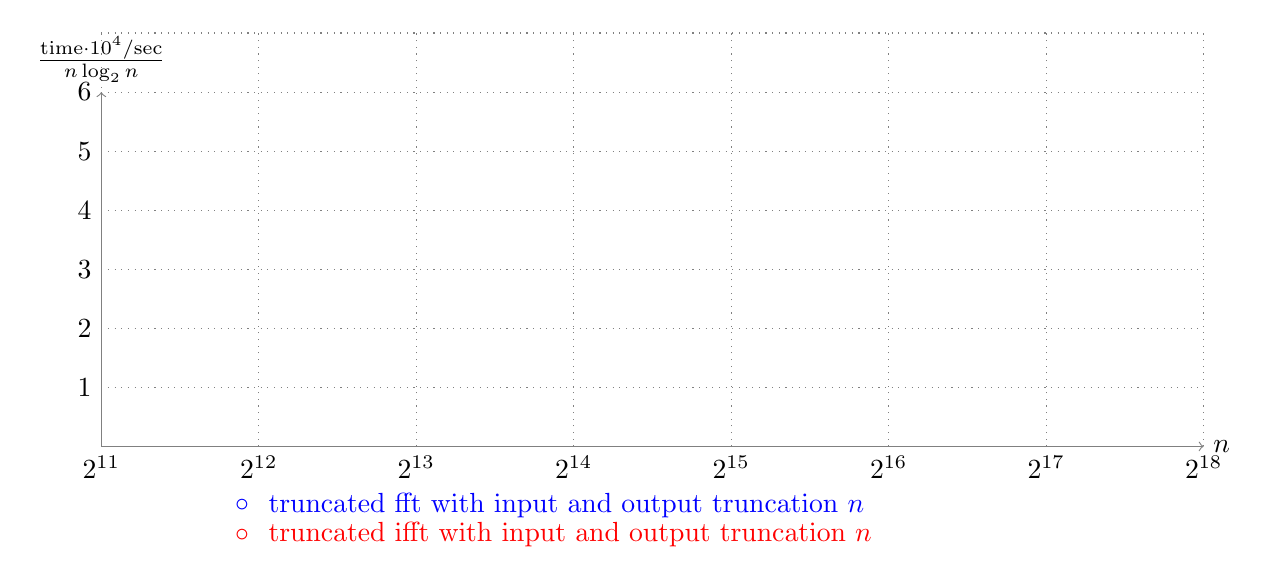
\begin{tikzpicture}[xscale=2.0, yscale=0.75]
\draw [dotted, gray] (11,0) grid (18,7);
\draw[latex-latex, thin, draw=gray, -to] (11,0)--(18,0) node [right] {$n$};
\draw[latex-latex, thin, draw=gray, -to] (11,0)--(11,6) node [above] 
{$\frac{\text{time} \cdot 10^{4}/\text{sec}}{n \log_2 n}$};
\foreach \p in {1,2,3,4,5,6}{\node [black] at (11,\p) [left] {$\p$};}
\foreach \p in {11,12,...,18}{\node [black] at (\p,0) [below] {$2^{\p}$};}
\foreach \p in \flinttruncblue{\node [blue] at \p {$\circ$};}
\foreach \p in \flinttruncred{\node [red] at \p {$\circ$};}
\node [blue] at (12,-1.0) [left] {$\circ$};
\node [blue] at (12,-1.0) [right] {truncated fft with input and output 
truncation $n$};
\node [red] at (12,-1.5) [left] {$\circ$};
\node [red] at (12,-1.5) [right] {truncated ifft with input and output 
truncation $n$};
\end{tikzpicture}
}
\end{figure}



\end{document}

